
% %\begin{abstract}
% Counter machines are a particularly simple, Turing-complete
% model of computation.
% We study the expressive power of nondeterministic
% counter machines which are symmetric, namely their
% transitions are invariant under swapping of counters.
% As the main result we demonstrate that symmetric 2-counter machines
% are not Turing-complete, by proving decidability of their 
% reachability problem.
% %Our approach builds on specific properties of 2-counter
% %machines, and does not extend to 3 or more counters.
% We conjecture the decidability 
% for nondeterministic machines with arbitrarily many counters,
% as long as (their transitions) are invariant under all permutations
% of counters. 
% We leave the status for symmetric 3-counter machines open, but
% identify a bound on the impact of symmetry by proving
% undecidabilty for 3-counter machines invariant under the
% cyclic permutation group.
% %\end{abstract}

\bigskip

\section{Introduction}

Counter machines (\cm{s}) are a particularly simple
model of computation \cite{Minsky67}.
A counter machine has a number of registers where it
stores its data, each register storing a natural number.
While the particular instruction sets may vary, 
common machine instructions are: counter increment, 
counter decrement, and counter zero-test. 
Many variants of the model have been introduced and studied,
and both deterministic and nondetermistic 
machines are widely studied in the literature 
(often under different names, for instance 
\emph{counter automata}).
Numerous syntactic restrictions of the model are also widely
studied \cite{HKOW09,Ibarra78,HopcroftPansiot,FS00}
since,
as shown already by Minsky in the early 1960s \cite{Minsky61},
in its full generality the model is Turing-complete:
deterministic 2-counter machines can faithfully simulate Tuting machines
and have undecidable halting problem. 

The purpose of this paper is to understand the impact of
\emph{symmetry} on the expressive power of \cm{s}. %counter machines.
We investigate the \emph{nondeterministic} model, where
a machine may choose between different istructions executable
in the same state.

\para{Symmetric counter machines}
As the starting point, we specifically choose the set of 
machine instructions:
counter \emph{updates} that simultaneously modify all counters  
by given numbers, and counter \emph{zero-tests} that are 
executable only if a given counter has value zero.
Every \emph{transition} $(q,i,q')$ of a machine changes its state
from $q$ to $q'$,
and executes an attached instruction $i$.
Executing a transition in a given configuration constitutes a 
\emph{step} of a machine.
The model we investigate is thus essentially \vass
(vector addition systems with states) \cite{HopcroftPansiot}
extended with zero-tests, and
is clearly equivalent to standard \cm{s}. %counter machines.
In this paper we mostly focus on \cm{s} %counter machines 
that are 
\emph{symmetric}, by which we mean that the set of transitions
is invariant under all permutations $\sigma$ of counters:
for every transition $(q,i,q')$, the machine has also a transition
$(q,\sigma(i), q')$, where $\sigma(i)$ is the result of 
applying $\sigma$ to the counters in the instruction $i$.
Specifically, we choose to impose the invariance only on update transitions
(when $i$ is a counter update), but
not on zero-test transitions, since the latter does not seems
necessary for our proofs to work.
Here is an illustrative example of a 2-\cm (a \cm having two counters)
with
two control states and
six transitions, including five symmetric update transitions
and one zero-test transition:
\sla{the example to be improved}
% \begin{figure}
\begin{center}
\scalebox{0.7}
{\begin{tikzpicture} [draw=black!70,
  fill=blue!20, node distance = 4cm, on grid, auto,
  every initial by arrow/.style = {thin}]
% State q0 
\node (q0) [state, scale=1.4, fill=blue!20, initial text = {}] {$p$};
% State q1  
\node (q1) [state, scale=1.4, fill=blue!20, right = of q0] {$q$};
% Arrows
\path [-stealth, thick]
   (q0) edge[bend left] node[scale=1.5] {\tiny{$\textbf{zero-test}_1$}}  (q1)
   (q1) edge[bend left] node[scale=1.1] {$(-1,-1)$}  (q0)
   (q0) edge [loop above] node[scale=1.5] {$\substack{(-1, 3) \\ (3, -1)}$}()
   (q1) edge [loop above] node[scale=1.5] {$\substack{(1, -1) \\ (-1, 1)}$}();
\end{tikzpicture}}
\end{center}
% \caption{A symmetric 2-counter machine.}
\label{fig:example}
% \end{figure}


\para{Contribution}
The initial motivation of this study is the immense impact of symmetry
on complexity of the \vass reachability problem:
while the problem is {\sc Ackermann}-complete in general \cite{LS19,CO21,L21},
the complexity drops to
only \pspace-complete for symmetric \vass \cite{KL25}.
As our main result, we confirm the immense drop in case of 
2-\cm{s}
(in this case, symmetricity amounts to invariance under all swaps of 
counters).
We prove decidability of the configuration-to-configuration reachability
problem, when one aks if a given machine has a sequence of steps
starting in a given source configuration and ending in
a given target one:

\begin{theorem} \label{thm:main}
The reachability problem  is decidable for symmetric 2-counter machines.
\end{theorem}

Symmetric two-counter machines are thus not Turing-complete.
We find this result quite surprising, as it applies to a model
with unrestricted zero-test instructions.

\begin{remark}
In the proof we do not need symmetry of zero-test transitions,
only symmetry of updating transitions.
Interestingly, the converse restriction, namely imposing symmetry on
zero-test transitions but not on update transitions immediately 
leads to undecidability.
\end{remark}

A natural question is whether \Cref{thm:main} extends to larger numbers of
counters. 
In particular, is the reachability problem still decidable
for symmetric 3-counter machines, whose update transitions are invariant
under all 6 permutations of the 3 counters?
Our decidability argument does not extend to the 3-counter setting, 
as the argument relies on a
number of low-dimensional properties of reachable sets and reachability
relations.
We thus leave this intriguing question for further research, conjecturing
decidability for any numner of counters:

\begin{conjecture}
The reachability problem  is decidable for symmetric counter machines.
\end{conjecture}

Another question we leave open is the exact complexity of the problem.
As the lower bound, we known nothing more than 
\pspace-hardness inherited from symmetric 2-\vass \cite{KL24}.
It is possible that the reachability problem is \pspace-complete
in symmetric $d$-\cm{s} for every $d\leq 2$.
\sla{expand}

\medskip

It is natural to consider invariance under certain subgroups
of permutations: for every subgroup $G\leq \symg d$
one can consider the class of \emph{$G$-counter machines}
($G$-\cm{s}), namely 
$d$-counter machines invariant under all permutations from $G$.
On one end, 
when $G=\symg d$, the general definition instantiates to 
symmetric $d$-\cm{s}.
On the opposite end, when $G$ is the trivial group one gets classical counter
machines.
Between the two extremities there is a landscape of models, 
whose expressive power is related according to the permutation subgroup relation:
whenever $G\leq H$, every $H$-\cm is automatically a
$G$-\cm.
For instance, every $\symg 3$-\cm is automatically
a $\cycg 3$-\cm, for the cyclic 
permutation group $\cycg 3 \leq \symg 3$.
As an additional result, we identify a bound on the impact of symmetry,
already for 3-counter machines, namely we prove undecidability 
for $\cycg 3$-counter machines:

\begin{theorem} \label{thm:undecid}
The reachability problem  is undecidable for $\cycg 3$-counter machines.
\end{theorem}


\para{Related research}

Identifying decidable restrictions of counter machines
is a very active line of research since 1960s, for instance 
1-counter, reversal-bounded, or restricted 2-counter machines 
\cite{HKOW09,Ibarra78,FS00}.
A prominent example is counter machines without zero-tests, that is
vector addition systems with states
(\vass), shown to have decidable reachability in early 1980s
\cite{Mayr81,Kosaraju82,Lambert92}.
The decidability extends to 
\cm{s}
with only one zero-tested counter \cite{Bonnet11},
or with with nested zero-tests \cite{Reinhardt08,GCL25}.
On the other hand, most of natural restrictions of the counter model
preserves Turing-completeness, as long as no constraint is imposed
on zero-tests.
For instance, considering deterministic \cm{s}, 
the reachability problem is still undecidable
in the subclass of \emph{reversible} \cm{s},
where the step relation is reverse deterministic, and hence every step
may be uniquely undone \cite{Morita96}.

In the special case of 1 counter, symmetric 1-\cm{s} coincide with 
general 1-\cm{s}.
Their reachability problem is \np-complete 
if transition updates are encoded in binary, and \nl-complete 
in unary encoding \cite{HKOW09}.

% (Symmetric) 2-counter machines are an extesion of (symmetric) 2-\vass by 
% zero-tests.
Restricting the use of zero-tests in 2-counter machines often
leads not only to decidability, but even 
to \pspace-completenss of the reachability problem.
Assuming binary encoding,
the \pspace-completeness has been obtained for 2-\vass 
\cite{Blondin15,BEFGHLMT21}
(assuming unary encoding, we have \nl-completeness \cite{ELT16}),
but also for the further restriction to symmetric 2-\vass \cite{KL24},
and for a relaxation of 2-\vass to 
2-counter machines with just one zero-tested counter \cite{FLS18}.
In all the three cases the reachability relation is effectively semilinear, which
is a key for obtaining the \pspace upper complexity bound, and which 
fails when the number of counters is at least 3 (even for 3-\vass) 
\cite{HopcroftPansiot}.
We do not know the exact complexity of symmetric 2-counter machines,
but it is possible that the complexity remains \pspace.
Furthermore, we do not know if the reachability relation of a
symmetric 2-counter machine is semilinear, but we believe it is so.

Contrarily to the avove-mentioned restrictions of zero-tests, 
our model leaves the zero-tests unrestricted, which makes
\Cref{thm:main} particularly interesting.
We conclude by recalling another recently obtained decidability result that
also does not assume any explicit restriction of zero-tests \cite{Dudenhefner22}.
% , and hence seems as surprising as our \Cref{thm:main}.
It amounts to observing that
the above-mentioned Turing-completeness of 
reversible counter machines seems to be very fragile with respect
to the choice of instruction set of a \cm.
As shown in \cite{Dudenhefner22},
for certain 
choice of instruction set, the Turing-complete model of 2-\cm{s}
becomes decidable under the reversibility restriction.
% 

\para{Outline} 
Afer we define the model in \Cref{sec:model}, the subsequent
\Cref{sec:outline,sec:sl,sec:targetpump} are devoted to the proof of
\Cref{thm:main}.
We proceed in a top-down manner, by consecutive reductions to more and
more basic properties. 
In \Cref{sec:outline} we provide the proof of \Cref{thm:main},
buidling on effective
semilinearity of reachability sets and relations in the underlying
symmetric 2-\vass.
Then in \Cref{sec:sl} we prove the effective semilinearity,
building on the central property of target (resp.~source) pumping
of symmetric 2-\vass, that is finally shown in \Cref{sec:targetpump}.
Finally, \Cref{sec:undecid} contains the proof of \Cref{thm:undecid}.


\section{Symmetric counter machines} \label{sec:model}

Let $d$ be a positive integer.
A \emph{$d$-counter machine} ($d$-\cm in short) 
$\mach$
is a finite-state automaton whose transitions
may perform two kinds of instructions,
namely update and zero-test \emph{instructions},
on $d$ \emph{counters}, namely nonnegative integer values
stored by $\mach$.
Formally, we define such a machine as 
$\mach = (Q,T)$, where $Q$ is a finite set of control states,
$T\subseteqfin Q\times\Instr\times Q$ is a finite set of 
\emph{transiitons} of $\mach$,
and the set $\Instr$ of \emph{istructions} is the union of
update instructions and zero-testing instructions:
\[
\Instr \ = \ \setof{\updinstr{w}}{w\in\Z^d} \ \cup \ 
\setof{\ztinstr{i}}{i\in d}.
\]
Execution of $\updinstr{w}$ amounts to adding
the vector
$w$ to the counters, and execution of 
$\ztinstr{i}$ amounts to checking if counter $i$
has value 0.
Formally, we define the semantics of $\mach$ by considering
its \emph{configurations} $c=(q,v) \in Q\times \N^d$ and
the step relation between configurations determined by 
transitions of $\mach$:
$(q,v) \step (q',v')$ if 

\begin{itemize}
\item 
$v' = v + w$,  for some  $(q,\updinstr{w},q')\in T$, or
\item  
$v' = v$ and $v(i)=0$, for some 
$(q,\ztinstr i, q')\in T$.
\end{itemize}

\noindent
We use the term $d$-\vass (vector addition system with states)
for a $d$-\cm without zero-test instructions.

The symmetric group $\symg d$ acts naturally on vectors in $\Z^d$
and hence also on update transitions:
for $\sigma\in \symg d$ and $t=(q,w,q')\in T$, we define
$\sigma(t)=(q,\sigma(w),q')$, where $\sigma(w)(\sigma(i))=w(i)$
for every $i\in\setto d$.
A $d$-\cm $\mach$ is \emph{symmetric} if its update transitions
are invariant under the natural action: for every $\sigma\in \symg d$ 
and $t\in T$, we have $\sigma(t)\in T$.
Importantly, 
we note that no restriction is imposed on zero-test transitons of $\mach$.
Therefore we assume, \mywlog, 
that every zero-test applies to a single counter.

In the sequel
we mostly focus on symmetric 2-\cm{s},
which are 2-\cm{s} whose set of transitions is invariant under the
swap of counters.

The reflexive-transitive closure $\step^*$ of $\step$ we call
the \emph{reachability relation} (between configurations).
The \emph{reachability problem} asks, given a \cm $\mach$ and two
its configurations, source $c$ and target $c'$, whether $c \step^* c'$
(in which case we say that $c'$ is \emph{reachable} from $c$).
A reachability certificate, namely any sequence $\rho$ of configurations
\[
c \ = \ c_0 \step c_1 \step \ldots \step c_n \ = \ c'
\]
related by the step relation,
we call a \emph{run} from configuration $c$ to $c'$.

% A 2-\vass $\V$ is symmetric if whenever it has a transition
% $q \xstep{(x_1,x_2)} q'$
% then it also has the transposed transition 
% $q \xstep{(x_2,x_1)} q'$.

% %
% A \emph{symmetric counter machine} with two counters (\sym 2-\cm) is a 
% counter machine whose \vass component (\ie, the \vass obtained by removing zero tests) is a symmetric \vass.
% Thus, transitions are symmetric,
% but zero tests need not be, and can distinguish the two counters.

% We prove that reachability in \sym 2-\cm is decidable.
% The proof consists of two independent sections:
% \cref{sec:targetpump}, which proves a general lemma about \sym 2-\cm{s},
% and \cref{sec:strategy,sec:proof}, which use that lemma (as a black-box)
% to prove the decidability result.


\section{Outline of decidability proof}\label{sec:outline}

% % As above, we use $\step$ to denote step relation of a 2-\vass, namely without zero tests.
% First some notational preprocessing.

Consider a symmetric 2-\cm $\mach = (Q,T)$ and 
two configurations, source $s$ and target $t$  ($s,t \in Q\times\N^2$).

\para{Decomposition of run into segments}
For convenience, we perform on $\mach$ the following notational
preprocessing:
we replace every zero-test transition
$t=(q,\ztinstr i, q')\in T$ by a sequence of two transitions,
\[
(q, \ztinstr i, q^t) \qquad
(q^t, \updinstr {0,0}, q'),
\]
% q \xstep{\textsf{c}_i=0?} S_i^t \xstep{(0,0)} q',\]
where $q^t$ is a new state, unique to the transition $t$.
Notice that reachability in the new symmetric 2-\cm thus obtained 
is equivalent to the original one, 
and that it has special states $q^t$
which can only be entered if the counter zero-tested by 
transition $t$ is zero;
we call them \emph{zero-testing states}.
The zero-testing states have the property
that they ``remember'' which counter is zero 
when the control of the machine is at them,
and that zero-test transitions are exactly those entering
a zero-testing state.
A fragment (infix) of a run between two consecutive zero-testing
states consists of only update transitions, except for the very last
transition which is a zero-test.
Such a fragment, called \emph{segment} in the sequel,
may be considered as a 2-\vass run
that ends with one counter 0, and which counter is 0 is
determined by the ending, zero-testing state.
Fornally, we will concider a segment as a run in the
\emph{unbderlying} symmetric 2-\vass $\V$
obtained by replacing every zero-test transition 
$(q, \ztinstr i, q^t)$ by
the corresponding $(0,0)$ update one
$(q, \updinstr{0,0}, q^t)$.

\begin{remark} \label{rem:wlog}
Furthermore, \mywlog we may assume that one counter is 0
in both source and target configurations.
For instance, if the source vector is $v=(v_1,v_2)$ with $0<v_1\leq v_2$,
we replace it by $(0,v_2-v_1)$ and add one extra transition
with update $(v_1,v_1)$.
We thus assume that the source and target states are zero-testing.
\end{remark}

%into those corresponding to counter $\textsf{c}_1$ and to counter $\textsf{c}_2$,
%so we tell which counter is zero by looking at the state.


% The strategy of the proof is to 
In the decidability proof we exploit the unique
decompostion of a run $\rho$ from source $s$ to
target $t$ 
into segments:
%\[ \rho=\rho_0 z_1 \rho_1 z_2 \dots \rho_{n-1}z_n\rho_n,\]
\[ \rho=\rho_0 \rho_1 \dots \rho_n,\]
where 
each $\rho_i$ starts and ends at consecutive zero-testing states of 
$\rho$.
% ---%
% we shall call the $\rho_i$ the \emph{\vass segments} of $\rho$.
%
Every $\rho_i$ is thus
a run in the underlying 2-\vass $\V$
of one of the following forms:
\begin{alignat}{2} 
  \begin{aligned} \label{eq:4cases}
q(a,0) &\step^\ast q'(0,a')\\
q(0,a) &\step^\ast q'(0,a')\\
q(0,a) &\step^\ast q'(a',0)\\
q(a,0) &\step^\ast q'(a',0),
  \end{aligned}
\end{alignat}
where the initial and final states $q$ and $q'$ are zero-testing states, and no zero-testing
state is visited in between.
Notice that we may write just
% \begin{equation*} %\label{eq:basictran}
$q(a) \step^* q'(a')$
% \end{equation*}
without specifying which of the four cases occurs,
since the (zero-testing) states $q$, $q'$ uniquely determine that.
We follow the notational shorthand %\eqref{eq:basictran} 
throughout and, instead of 
$\step^*$ which is a binary relation on $Q\times\N^2$,
%  \  \subseteq  (Q\times\N^2)^2$
we prefer to use 
a binary relation on $Q\times\N$, 
\[
\reachrel \ \ \subseteq \ (Q\times\N)^2,
\]
defined as expected: $q(a)\reachrel q'(a')$ if and only if 
any of the four cases of \eqref{eq:4cases} holds, namely
the underlying 2-\vass $\V$ has a corresponding run that does not
visit zero-testing states except for the initial and final ones.
% Without loss of generality, we also assume 
% that both the source and target vector have at least one 0.
Relying on Remark \ref{rem:wlog}, our taks is to decide if 
$s\reachrel^* t$
for $s,t\in Q\times\N$,
that is if the pair $(s,t)$ belongs to the reflexive-transitive
closure of $\reachrel$.

\begin{figure}
\centering
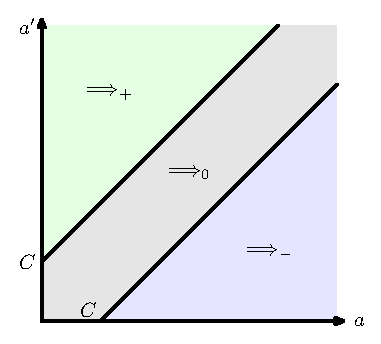
\includegraphics[scale=0.8]{figures-1.eps}
\caption{The three relations $\stepp +$, $\stepp -$, and $\stepp 0$.
The axes do \emph{not} correspond to the counters, 
but rather the initial and final values $a$ and $a'$ of a segment.}
\label{fig:areas}
\end{figure}


\para{Three types of segments}
Every segment $\rho_i \colon q(a) \reachrel q'(a')$, 
depending on the values of $a$, $a'$ and $a-a'$,
falls into one of three categories,
%split the relation $\step^\ast$ into three subrelations,
%which represent different kinds of \vass runs in $(Q\times\N^2)$:
denoted by $\stepp +$, $\stepp -$, and $\stepp 0$.
% We split the relation $\reachrel$ into three disjoint subrelations; 
% depending on the value of $a$, $a'$, and $a'-a$. 
If $q(a) \reachrel q'(a')$, we write:
\begin{equation}
\left.
\begin{aligned}\label{eq:tran0-+}
& q(a) \stepp 0\, q'(a'),\quad && \text{if\ \ $a\leq C$ or $a'\leq C$ or $|a'-a|\leq C $}\\
& q(a) \stepp - q'(a'),\quad && \text{if\ \ $a' > C$\ \ and\ \ $a > a'+C${}}\\
& q(a) \stepp + q'(a'),\quad && \text{if\ \ $a\phantom{'} > C$\ \ and\ \ $a' > a+C${}}
\end{aligned}\right\}
\end{equation}
See \Cref{fig:areas} for a graphical illustration.
% 
The precise definition of constant $C$ will be given in \Cref{sec:targetpump}.
Thus the rechability relation is 
\[
\reachrel^* \ = \ 
\big(\stepp 0 \ \cup \ \stepp - \ \cup \ \stepp + \big)^*,
\] 
an arbitrary composition
of the three sub-relations arbitrarily many times.
Note that the composition assures that \emph{control states match}.
% 
% \bigskip\noindent
Using this categorization 
we split the run $\rho$ into three \emph{phases} (possibly empty): 

\begin{itemize}
\item $\Phi_1$, which is the \emph{prefix} of $\rho$ and ends with the \emph{last} $\rho_i$ of the form $\stepp +$,
\item $\Phi_2$, which is an \emph{infix} of $\rho$ and consists only of $\rho_i$'s of the form $\stepp {0}^*$, 
\item $\Phi_3$, which is the remaining \emph{suffix} of $\rho$ starting 
with \emph{the first} $\rho_i$ of the form $\stepp -$.
% (followed by other \vass segments of the forms $\stepp -$ and $\stepp 0$).
\end{itemize}

\noindent
Clarly, the composition of the three phases yields
the reachability relation, that is
\begin{align} \label{eq:reachrel}
\reachrel^* \ = \ \Phi_1 \circ \Phi_2 \circ \Phi_3,
\end{align}
for  the three relations defined by the following rational expressions:
\begin{align*}
&\Phi_1 \ = \ ((\stepp 0 \ \cup \ \stepp -)^\ast \circ \stepp +)^\ast,\\
&\Phi_2 \ = \ (\stepp 0)^\ast,\\
&\Phi_3 \ = \ (\stepp - \circ \stepp {0}^\ast)^\ast.
\end{align*}

\para{Outline of decidability proof}

The proof uses semilinear sets.
Any subset of $\N^d$ of the form
\[
% \lin b {\{p_1,\dots,p_n\}} = 
\left\{ b + k_1 p_1 + \cdots + k_n p_n 
\mid k_1, \dots, k_n \in \N \right\},
\]
for $b, p_1, \dots, p_n \in \N^d$,
we call a
\emph{linear} set with base $b$ and periods $p_1, \dots, p_n$.
A \emph{semilinear} set is a finite union of linear sets in the same
dimension $d$.
We say $X \subseteq Q \times \N^d$ is semilinear 
if for every $q \in Q$, 
the set 
\(\{n \mid (q,n)\in X\} \subseteq \N^d\)
is semilinear.
Similarly, 
$R \subseteq (Q\times \N^d)^2$ is semilinear if for every $q,q' \in Q$,
the set
\( \{(n,n') \mid ((q,n),(q',n')) \in R \} \subseteq \N^{2d}\)
is semilinear.

\Cref{thm:main} is proved by showing that the relation $\Phi_2$, 
as well as
the image of relation $\Phi_1$ and pre-image of $\Phi_3$, are
\emph{effectively semilinear}, which means that they are 
semilinear sets and their descriptions are computable
given the underlying 2-\vass $\V$ and source and target
$s, t\in Q\times\N$.
Importantly, we only need to consider semilinar sets and relations
in dimension $d=1$.


\begin{lemma} \label{lem:0star}
$\Phi_2 \subseteq (Q \times \N)^2$ 
is an \emph{effectively semilinear} relation.
% The relation $\stepp {0}^*$ is effectively semilinear.
\end{lemma}


% \begin{lemma} \label{lem:compbackfor}
% One can compute 
% the set 
% $\big(\stepp - \ \circ \ \stepp {0}^*\big)^* \ \circ \ \{t\}$.
% \end{lemma}

\begin{lemma} \label{lem:compbackfor}
Given source $s$ and target $t$, the sets
\begin{alignat*}{6}
&\Phi_3 \circ \{t\} \ := \  \{y &&\mid (y,t) \in \Phi_3 \hskip 0.5pt\}  \ \subseteq \ Q \times \N, \\
&\{s\} \circ \Phi_1 \ := \  \{x &&\mid (s,x) \in \Phi_1 \} \ \subseteq \ Q \times \N
\end{alignat*}
are \emph{effectively semilinear}.
% One can compute 
% the set 
% $\{s\} \circ \big(\stepp {0}^* \ \circ \ E \ \circ \ \stepp +)^*$.
\end{lemma}

%  $\Phi_2 \subseteq (Q \times \N)^2$ 
% is an \emph{effectively semilinear} relation
% %\footnote{This means $\{n \in \N \colon (q,n) \in \Phi_3 \}$ is effectively semilinear, for every $q\in Q$.}%
% % 
% and that for given source $s$ and target $t$, the sets
% \begin{alignat*}{6}
% &\Phi_3 \circ \{t\} \ := \  \{y &&\mid (y,t) \in \Phi_3 \hskip 0.5pt\}  \ \subseteq \ Q \times \N, \\
% &\{s\} \circ \Phi_1 \ := \  \{x &&\mid (s,x) \in \Phi_1 \} \ \subseteq \ Q \times \N
% \end{alignat*}
% are also \emph{effectively semilinear}.

Relying on effective 
semilinearity given in \Cref{lem:0star,lem:compbackfor},
and on the effective equivalence of semilinear sets and Presburger 
Arithmetic \cite{},
the proof of \Cref{thm:main} is immediate:
the reachability question $s\reachrel^* t$
which, according to \eqref{eq:reachrel}, is equivalent to%
%\( (s,t) \in \Phi_1\circ\Phi_2\circ\Phi_3,\) \ie 
\begin{equation}
\exists\, x,y \in Q\times\N \ : \  x \in \{s\} \circ \Phi_1 \ \wedge \ (x,y) \in \Phi_2 
\ \wedge \ y\in \Phi_3 \circ \{t\},
\end{equation}
is effectively 
expressible in Presburger Arithmetic, and hence decidable \cite{}.
It thus remains to demonstrate the two key lemmas.


%Notationally, we allows ourselves to compose a relation $R\subseteq (Q\times\N)^2$ 
%with a set $X\subseteq Q\times\N$ to denote the set inverse image $R\circ X\subseteq Q\times\N$, 
%or the image $X\circ R \subseteq Q\times\N$.
%% Let $I_s = \{(s,s)\}$ be the relation containg exactly one pair, where $s$ is the source configuration.
%% Likewise, let $I_t = \{(t,t)\}$.
%We will be able to decide if $s\step^* t$, given source and target configurations $s,t\in Q\times\N$,
%as long as we prove the two following fact: one can (backward) compute the inverse image
%$E\circ \{t\}$, and (forward) compute the image 
%$\{s\} \circ \big(\stepp {0}^* \ \circ \ E \ \circ \ \stepp +)^*$,
%according to the partition into phases.




\section{Effective semilinearity} \label{sec:sl}

We denote by $\mysize \V$ the size of $\V$, in unary representation,
and by $\norm \V$ the max-norm of $\V$, namely the maximal absolute value of
all numbers appearing in transitions.
Clearly, $\mysize \V \geq \norm \V$.

We start with a basic observation concerning the building blocks
of sets of our interest:

\begin{lemma} \label{lem:0-+}
The relations $\stepp 0, \ \stepp -, \ \stepp +$ are effectively semilinear.
\end{lemma}
\begin{proof}
The relation $\reachrel$ is the reachability relation of a 2-\vass
$\V$, which is effectively semi-linear \cite{Blondin15}.
Each of the sub-relations $\stepp 0, \ \stepp -, \ \stepp +$ is a Presburger-definable subset of $\reachrel$,
and hence effectively semilinear as well.
\end{proof}


\para{Target and source pumping}


The \emph{target pumping} 
property of segments of the form $\stepp +$, is 
a central technical tool in the proofs of
\Cref{lem:0star,lem:compbackfor}:

\newcommand{\punkt}[2]{({#1}{\rightarrow}{#2})}
\begin{lemma} [Target pumping] \label{lem:targetpump}
Given a symmetric 2-\vass $\V$,
one can compute numbers $C, D \in \N$ 
such that for every pair of control states $q, q'$ of $\V$ and  
$a, a'\in\N$ such that $a > C$ and $a' > a + C$,%
\[
\punkt 1 2 \qquad
\text{if} \quad q(a,0)\step^* q'(0,a') \quad \text{then} \quad q(a,0) \step^* q'(0, a'+D),
\]
and similarly for the other three symmetric cases:
\begin{alignat*}{3}
&\punkt 2 2 \qquad
\text{if} \quad q(0,a)\step^* q'(0,a') \quad &&\text{then}  \quad  q(0,a) \step^* q'(0, a'+D),\\
&\punkt 2 1 \qquad
\text{if} \quad q(0,a)\step^* q'(a',0) \quad &&\text{then}  \quad  q(0,a) \step^* q'(a'+D, 0),\\
&\punkt 1 1 \qquad
\text{if} \quad q(a,0)\step^* q'(a',0) \quad &&\text{then}  \quad  q(a,0) \step^* q'(a'+D,0).
\end{alignat*}
Moreover, $C$ is polynomial in $\mysize \V$ and $D$ is exponential in $\mysize \V$.
\end{lemma}

In the sequel we fix the underlying symmetric 2-\vass $\V$ of
a symmetric 2-\cm.
The four claims of \Cref{lem:targetpump} jointly imply that 
$\stepp +$ is \emph{target-pumpable} in $\V$, 
that is for every pair of control states $q, q'$ of $\V$, 
% and  $a, a'\in\N$ such that $a, a'-a > C$, 
\begin{align} \label{eq:tpump}
q(a)\stepp + q'(a') \quad \implies  \quad  q(a) \stepp + q'(a'+D).
\end{align}
The reverse version of the four claims, where we swap source and target and reverse all transitions
(the reverse of $(q,w,q')$ is $(q',-w,q)$, as expected), 
implies that $\stepp -$ is \emph{source-pumpable}, that is 
\begin{align} \label{eq:spump}
q(a)\stepp - q'(a') \quad \implies  \quad  q(a+D) \stepp - q'(a').
\end{align}
Note that we can assume the same $D$ in \eqref{eq:tpump} and 
\eqref{eq:spump}, by taking the least common multiplicity of the
two constants given by the two applications of \Cref{lem:targetpump}.
In the sequel, fix the constant 
$D$ from \eqref{eq:tpump} and \eqref{eq:spump}.


\para{Periodic sets}

A set $X \subseteq Q \times \N$ is $N$-periodic if
for all $(q,a) \in X$, also $(q,a+N) \in X$.
It is a folklore that semilinear sets $X\subseteq Q\times\N$
are $N$-periodic for some period $N$. 
In the sequel it will be crucial that all semilinear sets we maintain
are $D$-periodic with the same period $D$.
% 
For instance, in consequence of \eqref{eq:tpump} and \eqref{eq:spump}, 
the image $S\circ \stepp +$ as well as the pre-image
$\stepp - \circ S$ is always $D$-periodic, irrespectively of
$S\subseteq Q\times\N$.
% 
%Now define the three phases $\Phi_1, \Phi_2, \Phi_3$ as stated above.
%
%\begin{align} \label{eq:3phases}
%\big(\stepp {0}^* \ \circ \ E \ \circ \ \stepp +)^* \ \circ \ \stepp {0}^* \ \circ \ E
%\end{align}
%where 
%\[
% E  \ = \ \big(\stepp - \ \circ \ \stepp {0}^*\big)^*.
%\]
%Thus we split every run into three phases: the first one ends with the last appearance of $\stepp +$,
%the middle one consisting just of $\stepp {0}^*$, and the last one starting with $\stepp -$ and
%iterating arbitratily many times $\stepp -$ and $\stepp 0$.
%Each of the phases may be empty.
% 

A $D$-periodic set $X$ is representable by a function 
$\minf X : Q\times \setfromto 0 {D-1} \to \N \cup \{\infty\}$ 
that maps a state $q\in Q$ and $r<D$ to the least number $n$ 
whose reminder modulo $D$ equals $r$, and such that $(q,n)\in X$ 
(and to $\infty$ if there is no such number):
\[
\minf X (q,r) \ = \ \min\{n : (q,n) \in X, \ \ n \equiv r\!\!\mod D\}.
\]
In the proofs of \Cref{lem:0star,lem:compbackfor}
we compute increasing (actually, non-decreasing) chains 
of $D$-periodic sets of configurations $X\subseteq Q\times\N$.
%We represent these sets in vector form as functions
%$X:Q\to \powset{\N}$, where $X(q)$ is pumpable for every $q\in Q$, namely $a\in X(q)\implies a+D\in X(q)$.
Termination of computation is guaranteed by:
%  the following lemma:
\begin{lemma} \label{lem:stab}
    Every non-decreasing chain of $X_1 \subseteq X_2 \subseteq \cdots$ of $D$-periodic sets of $\N$ stabilizes.
\end{lemma}
% 
\begin{proof}
The sequence $\minf {X_1}, \minf{X_2}, \ldots$ is a non-increasing
chain of functions, ordered pointwise 
(assuming $n<\infty$ for $n\in\N$), 
and hence necessarily stabilises due to well-foundedness
of the function space $Q\times \setfromto 0 {D-1} \to \N \cup \{\infty\}$.
\end{proof}


\begin{proof}[Proof of \Cref{lem:0star}]
    \vrm{Hard; to write down later.}\par
    Computable by a 1-counter automaton, a special case of a pushdown automaton.
\end{proof}

\begin{proof}[Proof of \Cref{lem:compbackfor}]
Recall that $\big(\stepp - \ \circ \ \stepp {0}^*\big) \ \circ \ S$
is the set of all 
\((q,a) \in Q \times \N\) such that $q(a)$ leads to some $x \in S$ via a run of form $(\stepp -\stepp {0}^\ast)^\ast$.
Thus, $\big(\stepp - \ \circ \ \stepp {0}^*\big) \ \circ \ S$ is source-pumpable 
due to \eqref{eq:spump},
irrespectively of $S$.

It is also computable due to \Cref{lem:0-+,lem:0star}, 
as long $S$ is semilinear.
This is seen by iterating the computation of the transformation
\[
S \quad \mapsto \quad \big(\stepp - \ \circ \ \stepp {0}^*\big) \ \circ \ S
\quad \cup \quad S,
\]
which stabilises, by \Cref{lem:stab}.
\vrm{how many details to write here? $\stepp {0}^\ast$ has a representation as a semilinear set;
to explain why every intermediate step in fixed point computation also has an efficient representation,
and give it.}
Furthermore, by the effective representation of $\stepp {0}^\ast$ and $\stepp {-}$ as semilinear relations,
each step of the process above is effectively representable,
and thus so is the fixed point.
\end{proof}

\begin{proof}[Proof of \Cref{lem:compbackfor}]
Again, The set $f(S) = S \ \circ \ \stepp {0}^* \ \circ \ E \ \circ \ \stepp +$ is
target-pumpable due to \eqref{eq:tpump},
irrespectively of $S$.
Computability is more involved, but relates again on iteration of the transformation
\[
S \quad \mapsto \quad f(S) \quad \cup \quad S,
\]
relying on \Cref{lem:stab}.

\vrm{To write that $f(S)$ consists of arithmetic progressions of period $D$,
and that we choose the minimal element of every arithmetic progression.}
To compute $f(S)$, one first establishes which remainders modulo $D$ appear in this set,
by applyting the transformation of \Cref{lem:compback} to the set 
$(\stepp + \ \circ \ M_k)$,
where $M_k$ contains all numbers equal to $k$ modulo $D$, and checking intersection with 
the set $(S\ \circ \ \stepp 0)$. 
Then, by exhaustive search one finds the smallest number in $f(S)$, 
for each remainder modulo $D$ separately.
\end{proof}
